%
% $XORP: xorp/docs/multicast/multicast_arch.tex,v 1.4 2002/12/11 10:19:33 pavlin Exp $
%

\documentclass[11pt]{article}

%\usepackage[dvips]{changebar}

\usepackage{subfigure}
\usepackage{fullpage}
\usepackage{setspace}         % XXX: enabling this may break the compilation
\usepackage{times}
\usepackage{latexsym}
\usepackage{psfig}
\usepackage{graphicx}
\usepackage{xspace}
\usepackage{color}
%\usepackage[dvipdf]{graphics}
%\usepackage[dvips]{graphicx}
%\usepackage{xorp}

\definecolor{gray}{rgb}{0.5,0.5,0.5}
\newcommand{\etc}{\emph{etc.}\xspace}
\newcommand{\ie}{\emph{i.e.,}\xspace}
\newcommand{\eg}{\emph{e.g.,}\xspace}
%\newcommand{\comment}[1]{{\color{gray}[\textsf{#1}]}}
\newcommand{\comment}[1]{}

% Changebar stuff
% \newenvironment{colorcode}{\color{blue}}{}
% \renewcommand{\cbstart}{\begin{colorcode}}
% \renewcommand{\cbend}{\end{colorcode}}

% \pagestyle{empty}

\begin{document}

\title{XORP Multicast Routing Design Architecture \\
\vspace{1ex}
Version 0.1}
\author{ XORP Project					\\
	 International Computer Science Institute	\\
	 Berkeley, CA 94704, USA			\\
	 {\it feedback@xorp.org}
}
\date{December 11, 2002}

\maketitle

\thispagestyle{empty}


%%%%%%%%%%%%%%%%%%%%%%%%%%%%%%%%%%%%%%%%%%%%%%%%%%%%%%%%%%%%%%%%%%%%%%%
\section{Introduction}


%%%%%%%%%%%%%%%%%%%%%%%%%%%%%%%%%%%%%%%%%%%
\subsection{Overview}

This document provides an overview of the XORP multicast architecture.
Routing Daemon. It is intended to provide a starting point for software
developers who wish to modify the multicast-related software.

XORP multicast architecture consists of user-level software
implementation of multicast routing protocols such as PIM-SM and IGMP.
This document provides an overview of the interaction among them,
as well as the interaction with the underlying multicast forwarding
engine and other parts of the system.

Similar to the other parts of the XORP architecture, the multicast
architecture is also based on modularity and abstraction.
In particular, there is one process per protocol, and each process
typically communicates with other processes by using XRLs, the XORP
inter-process communication mechanism~\cite{xorp:xrl}.

%%%%%%%%%%%%%%%%%%%%%%%%%%%%%%%%%%%%%%%%%%%
\subsection{Acronyms}

Acronyms used in this document:

\begin{itemize}

  \item {\bf MFC}: {\bf M}ulticast {\bf F}orwarding {\bf C}ache: another
  name for an entry in the multicast forwarding engine (typically used
  on UNIX systems).

  \item {\bf MFEA}: {\bf M}ulticast {\bf F}orwarding {\bf E}ngine
  {\bf A}bstraction

  \item {\bf MLD/IGMP}: {\bf M}ulticast {\bf L}istener {\bf D}iscovery/{\bf
  I}nternet {\bf G}roup {\bf M}anagement {\bf P}rotocol

  \item {\bf MRIB}: {\bf M}ulticast {\bf R}outing {\bf I}nformation
  {\bf B}ase

  \item {\bf PIM-SM}: {\bf P}rotocol {\bf I}ndependent {\bf M}ulticast--{\bf
  S}parse {\bf M}ode

  \item {\bf RIB}: {\bf R}outing {\bf I}nformation {\bf B}ase

\end{itemize}


%%%%%%%%%%%%%%%%%%%%%%%%%%%%%%%%%%%%%%%%%%%%%%%%%%%%%%%%%%%%%%%%%%%%%%%
\section{Protocol Abstraction}

Similar to the rest of the XORP architecture, XORP multicast routing
architecture is designed such that each of the implemented protocols
can be used for both real-world routing and for network simulations.  A
simulation can be composed of several (UNIX) processes, one per
protocol entity controlled by a single process, or all protocol entities
running within a single process. For debugging purpose the latter may be
simpler to use and control. Further, the all-in-one model might be more
scalable. The implication of this is that a protocol implementation
must not keep any global state.

In routing, the concept of a network port or interface is essential in a
sense that a routing protocol entity communicates with the rest of the
world through such ports/interfaces (think of this as a protocol entity
having several virtual interfaces and each virtual interface corresponds
to a physical interface, and those interfaces are used for
sending/receiving control messages to/from other routers). In case of
PIM for example, the routing entity has several virtual interfaces one
per each physical interface it controls.  In case of BGP,
the routing entity has several ports, one per each BGP peering.

In term of C++ coding, each virtual interface is a class; each protocol
entity is a separate class: a single protocol object has several virtual
interfaces (see Figure~\ref{fig:mcast_proto_abstraction}).

\begin{figure}[htbp]
  \begin{center}
    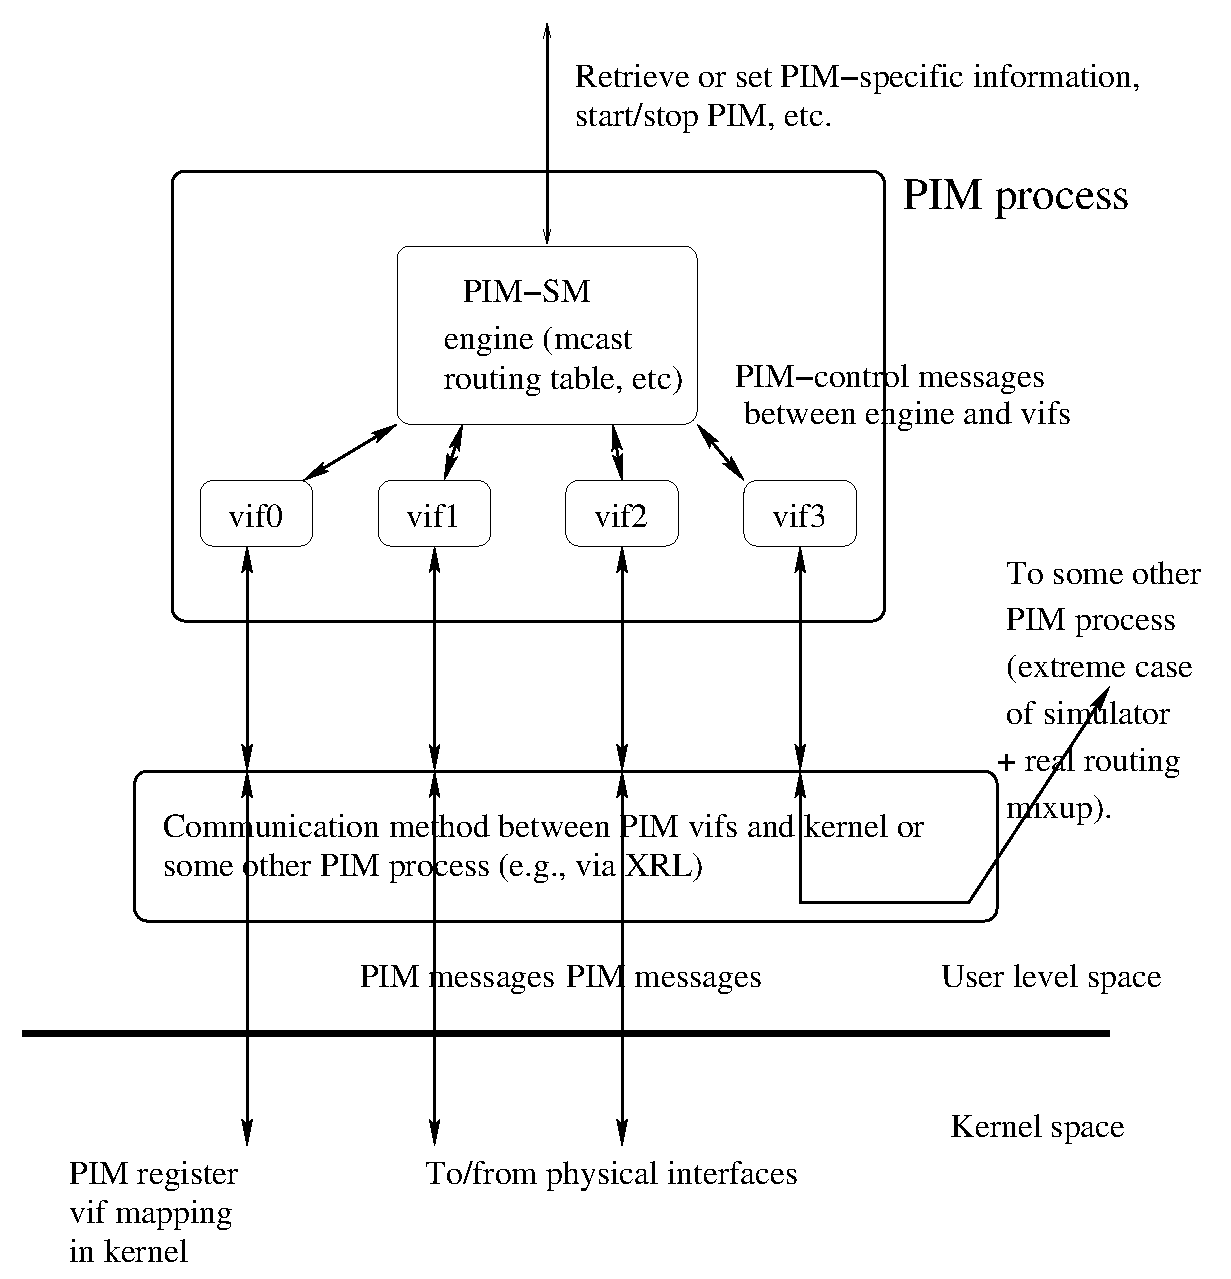
\includegraphics[width=5.0in]{figs/mcast_proto_abstraction}
    \caption{Multicast protocol abstraction}
    \label{fig:mcast_proto_abstraction}
  \end{center}
\end{figure}

At the protocol level implementation, the virtual interfaces do not
posses knowledge about the particular communication method used to send
or receive packets. To achieve this, the implementation uses pure
virtual C++ class methods (\eg methods declared such as:
{\it virtual int send() = 0;}).
The declaration of such methods require that each class must be
inherited by a ``wrapper'' class that implements all pure virtual
methods. Then, all the details about the particular mechanism
that is used to send or receive packets are in this wrapper class.
For example, that class might use XRLs, but it could be any other
mechanism that the developer provides (\eg a third-party simulation
testbed environment).

Such abstraction makes it very easy to reuse the protocol-specific code
for any other purpose, or to create several virtual ``nodes'' each of
them running the particular protocol. Those nodes can be either within
the same (UNIX) process or each of them running as a separate process,
as long as we have the right mechanism that allows them to communicate
with each other.

%%%%%%%%%%%%%%%%%%%%%%%%%%%%%%%%%%%%%%%%%%%%%%%%%%%%%%%%%%%%%%%%%%%%%%%
\section{MLD6/IGMP Daemon/Library}

Because a physical interface is owned by a single multicast routing
protocol, then we can have MLD6/IGMP running as a library on each of the
interfaces owned by that protocol. This solution may not work only if
there are more than one protocols that need membership information on an
interface.

The alternative solution is to have a separate MLD6/IGMP daemon that
takes care of membership per all interfaces, and then reports that
information to all interested parties. This will allow reporting this
information to more than one protocols per interface (in case we need
so).

Separating IGMP/MLD6 from the router code has the advantage of reducing
dependency and better robustness; \eg if the MLD6/IGMP code crashes, it
will not crash the routing protocol as well. Further, when it comes to
upgrade (\eg from IGMPv2 to IGMPv3), if we are running MLD6/IGMP as a
single process, then the upgrade can be performed by starting a new
MLD6/IGMP daemon on the place of the old one. This restart will not
require stopping the PIM daemon for example, which is very important for
routers in real-world operation.

%%%%%%%%%%%%%%%%%%%%%%%%%%%%%%%%%%%%%%%%%%%%%%%%%%%%%%%%%%%%%%%%%%%%%%%
\section{Multicast Modules Interaction}

\begin{figure}[htbp]
  \begin{center}
    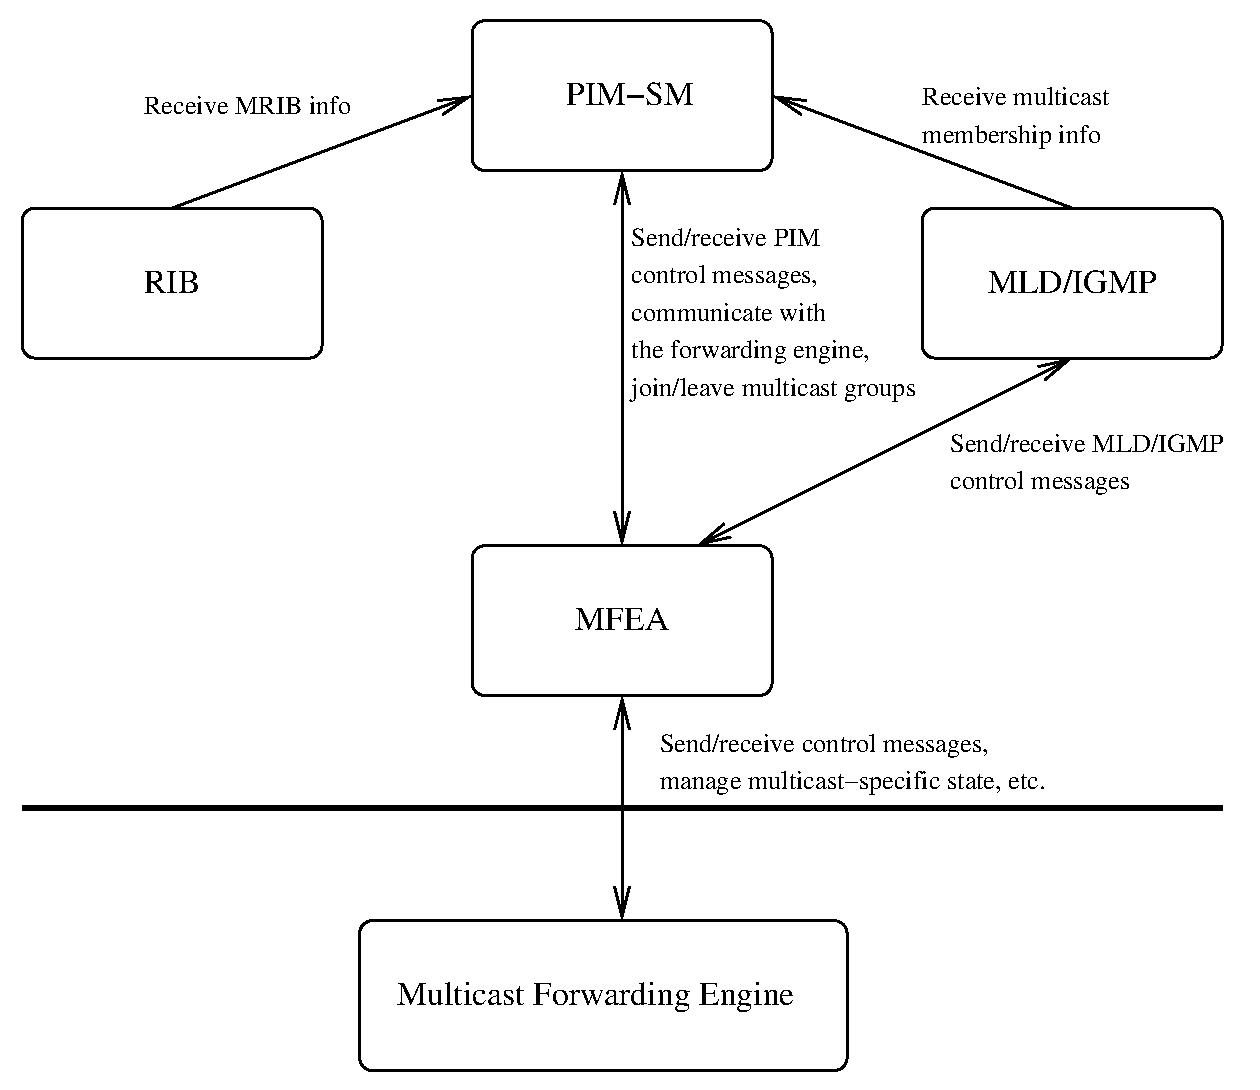
\includegraphics[scale=0.5]{figs/mcast_modules_interaction}
    \caption{Multicast Modules Interaction}
    \label{fig:mcast_modules_interaction}
  \end{center}
\end{figure}

Figure~\ref{fig:mcast_modules_interaction} shows the interaction among
the multicast-related modules. Those interactions are:

\begin{itemize}

  \item MFEA--PIM: to send or receive PIM control messages, to forward
   PIM-related signals from the multicast forwarding engine to PIM, to
   establish the communication between PIM and the multicast-forwarding
   engine, for the MFEA to join or leave a multicast group on behalf of
   PIM, etc.

  \item MFEA--MLD/IGMP: to send or receive MLD/IGMP control
  messages, and to join or leave a multicast group on behalf of
  MLD/IGMP.

  \item MLD/IGMP--PIM: for PIM to monitor multicast membership about
  local members.

  \item RIB--PIM: for PIM to obtain MRIB information.

\end{itemize}

In the next subsections we describe those interactions.

%%%%%%%%%%%%%%%%%%%%%%%%%%%%%%%%%%%%%%%%%%%
\subsection{Interaction between the MFEA and PIM modules}

PIM-SM needs to interact with the MFEA module for the following:

\begin{itemize}

  \item Send and receive PIM control messages.

  \item Start/stop the multicast forwarding engine.

  \item Add/delete multicast interface in the multicast forwarding
  engine.

  \item Add/delete multicast forwarding entry in the multicast
  forwarding engine.

  \item Receive PIM-related signals from the multicast forwarding engine
  (when applicable). Examples of such signals are NOCACHE or WRONGVIF
  on UNIX system to indicate that a multicast packet is received but
  there is no matching forwarding entry, or a packet was not received on
  the expected incoming interface respectively.

  \item Receive bandwidth-related information about multicast data
  flows: \eg whether a data flow is idle, or whether the bandwidth of a
  data flow is above a pre-defined threshold (need by PIM-SM to perform
  bandwidth-based Shortest-Path switch toward a source).

  \item Join/leave a multicast group.

  \item Currently (December 2002), the MRIB information is
  obtained through the MFEA.

  \item Currently (December 2002), the information about
  existing interfaces on a router is obtained through the MFEA.

\end{itemize}

On startup, the PIM module registers with the MFEA. As part of this
registration, the MFEA initiates sending of information about existing
interfaces on the system, and the current unicast forwarding
information. If any of this information changes later, the MFEA sends
the appropriate update to PIM. In addition, the MFEA creates the
appropriate state to send and receive PIM control messages. After the
PIM module receives the network interface information, it instructs the
MFEA to start PIM operation on selected interfaces. After that the PIM
module can send and receive PIM control messages on those interfaces.
Also, it it can send requests to the MFEA to add or modify multicast
forwarding entries in the kernel.

Note that the current (December 2002) solution for PIM kernel
uses one more signal from the kernel to the user-level daemon:
{\emph WHOLEPKT} messages. Those messages are multicast packets that are
suppose to be encapsulated in a PIM-SM Register message and sent to the
RP. The encapsulation mechanism must know the RP address (in general,
per multicast group address), and to avoid putting the RP addresses in
the kernel (which would also change the traditional multicast API), the
default solution is to use user-level encapsulation.  For best
performance, the PIM encapsulation should be done in the kernel, and
then we need a signaling mechanism between the kernel and the user
process managing the kernel multicast forwarding entries. That mechanism
will deal with installing the right information for kernel-level
Register encapsulation. Currently, there exist FreeBSD patches that
support such kernel-level encapsulation, and they will be added to
FreeBSD-CURRENT in January 2003.

%%%%%%%%%%%%%%%%%%%%%%%%%%%%%%%%%%%%%%%%%%%
\subsection{Interaction between the MFEA and MLD/IGMP modules}

MLD/IGMP needs to interact with the MFEA module for the following:

\begin{itemize}

  \item Send and receive MLD/IGMP control messages.

  \item Join/leave a multicast group.

  \item Currently (December 2002), the information about
  existing interfaces on a router is obtained through the MFEA.

\end{itemize}

On startup, the MLD/IGMP module registers with the MFEA. As part of this
registration, the MFEA initiates sending of information about existing
interfaces on the system, and the current unicast forwarding information. If
any of this information changes later, the MFEA sends the appropriate update
to MLD/IGMP. In addition, the MFEA creates the appropriate state to send and
receive MLD/IGMP control messages. After the MLD/IGMP module receives the
network interface information, it instructs the MFEA to start MLD/IGMP
operation on selected interfaces. After that the MLD/IGMP module can send and
receive PIM control messages on those interfaces.

%%%%%%%%%%%%%%%%%%%%%%%%%%%%%%%%%%%%%%%%%%%
\subsection{Interaction between the MLD/IGMP and PIM modules}

PIM-SM needs to interact with the MLD/IGMP module to receive multicast
membership information about local members. On startup, the PIM module
registers with the MLD/IGMP module by expressing interest tracking
multicast membership on selected network interfaces. After that, if
the multicast membership on any of the selected interfaces changes, the
MLD/IGMP module informs the PIM module about the change: \eg ``add
membership for group 224.0.1.20 on interface vif0''.

Note that control messages used for multicast debugging such as MRINFO or
multicast traceroute use IGMP as the network protocol. Hence, if such
messages are received by the MLD/IGMP module, the appropriate
information should be sent to the PIM module. Currently (December 2002),
the handling of such messages is not implemented yet. 

%%%%%%%%%%%%%%%%%%%%%%%%%%%%%%%%%%%%%%%%%%%
\subsection{Interaction between the RIB and PIM modules}

The PIM module needs to interact with the RIB module to obtain the MRIB
information, and to keep track if there is any change.
Currently (December 2002), this interaction is not implemented;
instead, the MRIB information is received from the MFEA instead.


%%%%%%%%%%%%%%%%%%%%%%%%%%%%%%%%%%%%%%%%%%%%%%%%%%%%%%%%%%%%%%%%%%%%%%%
%     APPENDIX
%%%%%%%%%%%%%%%%%%%%%%%%%%%%%%%%%%%%%%%%%%%%%%%%%%%%%%%%%%%%%%%%%%%%%%%
\appendix
\section{Modification History}

\begin{itemize}

  \item December 11, 2002: Version 0.1 completed.

\end{itemize}


%%%%%%%%%%%%%%%%%%%%%%%%%%%%%%%%%%%%%%%%%%%%%%%%%%%%%%%%%%%%%%%%%%%%%%%
%     BIBLIOGRAPHY
%%%%%%%%%%%%%%%%%%%%%%%%%%%%%%%%%%%%%%%%%%%%%%%%%%%%%%%%%%%%%%%%%%%%%%%
\bibliography{../tex/xorp}
\bibliographystyle{plain}

%%%%%%%%%%%%%%%%%%%%%%%%%%%%%%%%%%%%%%%%%%%%%%%%%%%%%%%%%%%%%%%%%%%%%%%
\end{document}
